\documentclass[11pt,a4paper]{article}
	% basic article document class
	% use percent signs to make comments to yourself -- they will not show up.

\usepackage{caption} %supress numbering figure from caption
\usepackage{hyperref}
\usepackage{tikz}
\usepackage{amsmath}
\usepackage{amssymb}
	% packages that allow mathematical formatting
\usepackage{float}
\usepackage{graphicx}
	% package that allows you to include graphics

\usepackage{setspace}
	% package that allows you to change spacing

\onehalfspacing
	% text become 1.5 spaced
\usepackage{wasysym} % contains the desired symbols

\usepackage{fullpage}
	% package that specifies normal margins

\usepackage{fancyhdr}
\pagestyle{fancy}
\lhead{\textbf{Solutions}}
\rhead{                                                   }
%\lfoot{Lecture 1}
%\rfoot{Handout 1}




\setlength{\headheight}{14pt}

% Solution blocks (same style as the Class 13 solutions)
\usepackage[most]{tcolorbox}
\definecolor{solblue}{RGB}{20,70,130}
\newtcolorbox{solution}{breakable, enhanced, blanker,
  left=10pt, top=2pt, bottom=2pt, before skip=6pt, after skip=10pt,
  borderline west={2pt}{0pt}{solblue}, colupper=solblue,
  before upper={\textbf{Solution.}\ }}

% Isocost lines (redrawn from Goolsbee et al., Microeconomics, 3e).
% C = WL + RK with W = $10, R = $20, so K = C/R - (W/R)L and the slope is -W/R = -0.5.
\definecolor{isogreen}{RGB}{0,166,118}
\newcommand{\isocostfigure}{%
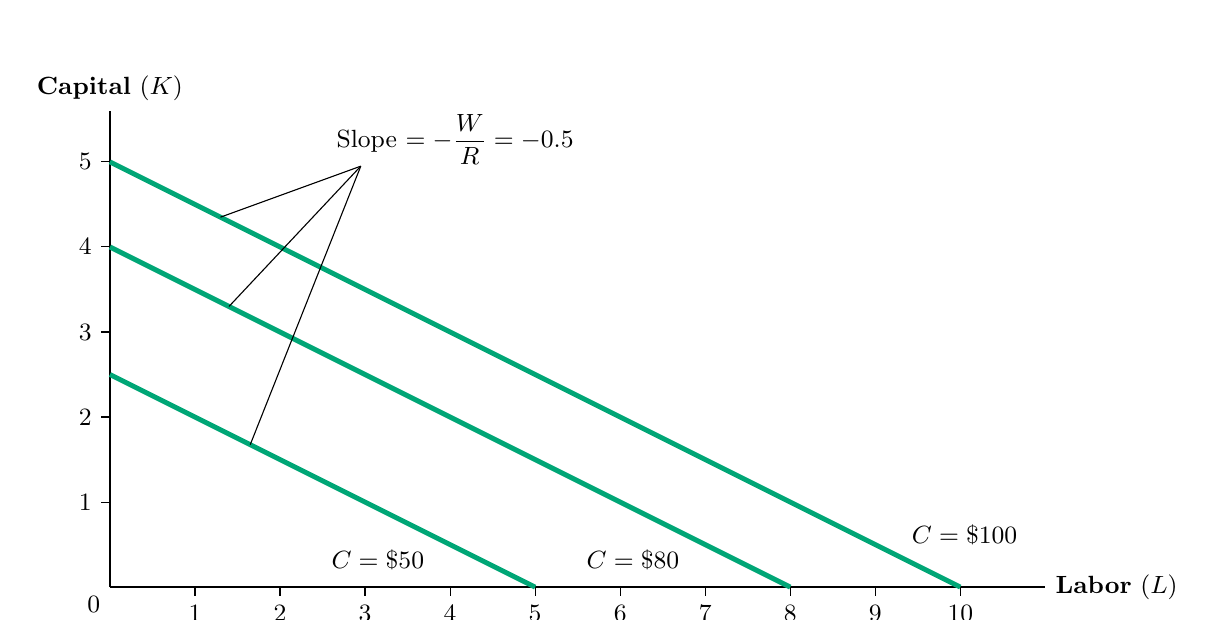
\begin{tikzpicture}[x=1.08cm,y=1.08cm,font=\small]
  % axes and ticks
  \foreach \x in {1,...,10} \draw (\x,0) -- (\x,-0.1) node[below] {\x};
  \foreach \y in {1,...,5} \draw (0,\y) -- (-0.1,\y) node[left] {\y};
  \node[below left] at (0,0) {0};
  \draw[thick] (0,0) -- (11,0) node[right] {\textbf{Labor} ($L$)};
  \draw[thick] (0,0) -- (0,5.6) node[above] {\textbf{Capital} ($K$)};
  % isocost lines
  \draw[line width=1.8pt,isogreen] (0,2.5) -- (5,0);
  \draw[line width=1.8pt,isogreen] (0,4) -- (8,0);
  \draw[line width=1.8pt,isogreen] (0,5) -- (10,0);
  \node at (3.15,0.32) {$C = \$50$};
  \node at (6.15,0.32) {$C = \$80$};
  \node at (10.05,0.62) {$C = \$100$};
  % slope label
  \node[anchor=south west] at (2.55,4.85) {Slope $= -\dfrac{W}{R} = -0.5$};
  \draw (2.95,4.95) -- (1.3,4.35);
  \draw (2.95,4.95) -- (1.4,3.3);
  \draw (2.95,4.95) -- (1.65,1.675);
\end{tikzpicture}}

% Cost curves for the Question 2 solution, drawn from one cost function so that
% MC crosses AVC and ATC exactly at their minima:
%   VC = 8Q - 2.4Q^2 + 0.32Q^3,  FC = 11.51104
%   MC  = 8 - 4.8Q + 0.96Q^2      (min at Q = 2.5,  MC  = 2)
%   AVC = 8 - 2.4Q + 0.32Q^2      (min at Q = 3.75, AVC = 3.5     -> shutdown point)
%   ATC = AVC + FC/Q              (min at Q = 4.6,  ATC = 6.2336  -> break-even point)
\definecolor{supplyorange}{RGB}{245,160,60}
\newcommand{\costfigure}{%
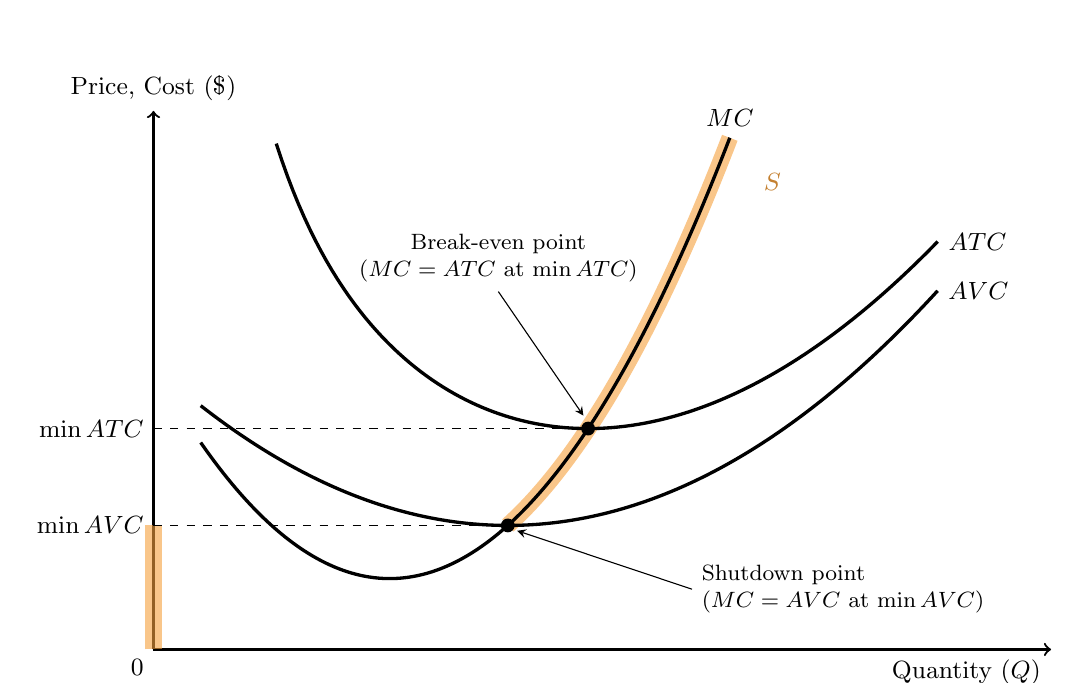
\begin{tikzpicture}[x=1.2cm,y=0.45cm,font=\small]
  % axes
  \draw[thick,->] (0,0) -- (9.5,0) node[below left] {Quantity ($Q$)};
  \draw[thick,->] (0,0) -- (0,15.2) node[above] {Price, Cost (\$)};
  \node[below left] at (0,0) {0};
  % short-run supply (shaded): Q = 0 below min AVC, MC above min AVC
  \draw[line width=6pt,supplyorange,opacity=0.6] (0,0) -- (0,3.5);
  \draw[line width=6pt,supplyorange,opacity=0.6,domain=3.75:6.1,samples=60]
    plot (\x,{8-4.8*\x+0.96*\x*\x});
  % price levels at the two points
  \draw[dashed] (0,3.5) node[left] {$\min AVC$} -- (3.75,3.5);
  \draw[dashed] (0,6.2336) node[left] {$\min ATC$} -- (4.6,6.2336);
  % cost curves
  \draw[very thick,domain=1.3:8.3,samples=120] plot (\x,{8-2.4*\x+0.32*\x*\x+11.51104/\x})
    node[right] {$ATC$};
  \draw[very thick,domain=0.5:8.3,samples=120] plot (\x,{8-2.4*\x+0.32*\x*\x})
    node[right] {$AVC$};
  \draw[very thick,domain=0.5:6.1,samples=120] plot (\x,{8-4.8*\x+0.96*\x*\x})
    node[above] {$MC$};
  \node[supplyorange!80!black,font=\small\bfseries] at (6.55,13.2) {$S$};
  % points
  \fill (3.75,3.5) circle (2.5pt);
  \fill (4.6,6.2336) circle (2.5pt);
  \draw[->,>=stealth] (5.7,1.7) node[right,align=left,font=\footnotesize]
    {Shutdown point\\($MC = AVC$ at $\min AVC$)} -- (3.85,3.35);
  \draw[->,>=stealth] (3.65,10.1) node[above,align=center,font=\footnotesize]
    {Break-even point\\($MC = ATC$ at $\min ATC$)} -- (4.55,6.6);
\end{tikzpicture}}

\begin{document}
\title{Class 14 Quiz Solutions}
\author{PUBPOL 205}
\date{October 15, 2026}
\maketitle
\thispagestyle{fancy}
\begin{enumerate}
\item The graph below shows three isocost lines for a firm that hires labor ($L$) at wage $W$ and rents capital ($K$) at rental rate $R$. Is labor more expensive, or is capital more expensive? Why?
\begin{center}
\isocostfigure\\[2pt]
{\footnotesize Adapted from Goolsbee et al., \textit{Microeconomics}, 3e.}
\end{center}

\begin{solution}
\textbf{Capital is more expensive.} An isocost line is the set of bundles that cost the same total amount, $C = WL + RK$. Solving for $K$:
\[
K = \frac{C}{R} - \frac{W}{R}\,L .
\]
The slope is minus the price of labor relative to the price of capital. Here $-W/R = -0.5$, so $W = 0.5R$: one unit of labor costs half as much as one unit of capital. Equivalently, one unit of capital costs as much as two units of labor. Along an isocost line, hiring one more unit of labor at the same total cost means giving up half a unit of capital.

Check with the intercepts of the $C = \$100$ line: \$100 buys 10 units of labor, so $W = \$10$, or 5 units of capital, so $R = \$20$. Then $W/R = 10/20 = 0.5$.
\end{solution}

\newpage
\thispagestyle{plain}
\item Consider a perfectly competitive firm in the short run. On the axes below, draw the firm's marginal cost ($MC$), average variable cost ($AVC$), and average total cost ($ATC$) curves, and sketch out the firm's short-run supply curve. Where is the break-even point? Where is the shutdown point? Label both on your graph.
\begin{center}
\costfigure
\end{center}

\begin{solution}
\begin{itemize}\setlength{\itemsep}{0pt}
\item \textbf{The curves.} $MC$ crosses both $AVC$ and $ATC$ at their minimum points: when $MC$ is below an average, one more unit pulls the average down, and when $MC$ is above it, one more unit pulls it up. Formally, $d(VC/Q)/dQ = (MC - AVC)/Q$, which is zero exactly where $MC = AVC$ (same for $ATC$). $ATC$ lies above $AVC$ by $AFC = FC/Q$, which shrinks as $Q$ grows, so the curves get closer and $\min ATC$ lies above and to the right of $\min AVC$.
\item \textbf{Break-even point:} where $MC = ATC$, at the minimum of $ATC$. At $P = \min ATC$ the firm produces where $P = MC = ATC$ and earns zero economic profit; above this price it earns a profit, below it a loss.
\item \textbf{Shutdown point:} where $MC = AVC$, at the minimum of $AVC$. If $P < \min AVC$, revenue does not cover variable cost, so producing loses more than shutting down (which loses only $FC$). The firm produces $Q = 0$.
\item \textbf{Short-run supply curve} (shaded): the firm sets $P = MC$, so supply is the $MC$ curve above $\min AVC$. For prices below $\min AVC$, $Q = 0$ (the shaded part of the vertical axis).
\item \textbf{Between the two points} ($\min AVC \le P < \min ATC$), the firm keeps producing at a loss: revenue covers all variable cost and part of fixed cost, so the loss is smaller than $FC$. Example: $FC = \$40$, $P = \$8$, and at the output where $P = MC$, $Q = 10$, $AVC = \$6$, $ATC = \$10$. Producing gives profit $(8 - 10) \times 10 = -\$20$; shutting down gives $-\$40$. Produce.
\end{itemize}
\end{solution}
\end{enumerate}
\end{document}
